\section{DC Servomotor}\label{sec:servo_motor}

The current legislation prevents the people to control UAVs out of the line of sight, which means that the users need to see the aircraft when they are piloting it. However, this legislation will change and it will be possible to control this device using a camera and a system which allows the communication between the ground station and the UAV. This connection between the antennas that are installed on both devices needs, thus, to be improved. So that, it will be necessary to develop a system able to control both antennas to put them pointing at each other.

In order to control both antennas, it is necessary to use motors which will be able to change its orientation. In this project, the DC servomotor was chosen because it can be either a rotary or a linear actuator which allows a precise control of angular or linear position, velocity and acceleration. The servomotor is basically constituted by a motor coupled to a sensor responsible for the position feedback. As a result, this motor requires a sophisticated controller designed specifically for servomotors.

Generally, a DC motor is an actuator which converts electrical energy to mechanical rotation. In the figure \ref{DC_servomotor_circuit} it is possible to see the model of a DC servomotor. The resistance and the inductance are responsible for the stability of the system. The equations \ref{DC_servomotor_equation1} and \ref{DC_servomotor_equation2} are the time and the frequency description of the circuit.

\begin{figure}[H]
\centering
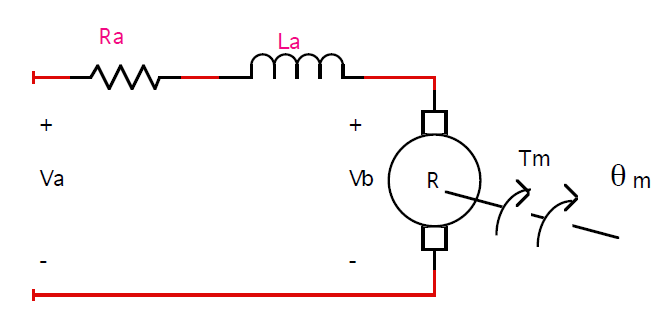
\includegraphics[scale=0.5]{figures/servomotor.png}
\caption{DC servomotor}
\label{DC_servomotor_circuit}
\end{figure}

\begin{equation}\label{DC_servomotor_equation1}
v_{a}= v_{b}+i_{a} R_{a}+L_{a}\frac{\mathrm{d} i_{a}}{\mathrm{d} t}
\end{equation}

\begin{equation}\label{DC_servomotor_equation2}
V_{a}(s)= V_{b}(s)+I_{a}(s) R_{a}+sL_{a}I_{a}(s)
\end{equation}

\begin{equation}\label{DC_servomotor_equation3}
I_{a}(s)= \frac{V_{a}(s)-V_{b}(s)}{R_{a}+sL_{a}} , I_{a}(s)= G_{I}(V_{a}(s)-V_{b}(s))
\end{equation}

\begin{figure}[H]
\centering
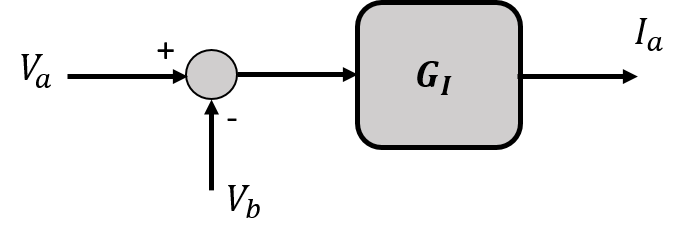
\includegraphics[scale=0.6]{figures/model1.png}
\caption{DC servomotor}
\label{model1}
\end{figure}

On the other hand, the sum of torques applied on the motor depends on the load attached to the motor shaft. The inertial and damping behaviours of the load can be represented as a inertia coefficient, $J_{e}$, and a viscous damping coefficient, $D_{e}$. This total tendency of a force to rotate an object about an axis is represented by $T_{m}$ which is described through the equations \ref{torque_time} and \ref{torque_frequency_theta}.

\begin{equation}\label{torque_time}
T_{m}(t)= J_{e}\frac{\partial^2 \theta_{m}(t)}{\partial t^2}+D_{e}\frac{\mathrm{d} \theta_{m}(t)}{\mathrm{d} t}
\end{equation}

\begin{equation}\label{torque_frequency_theta}
T_{m}(s)= (s^{2}J_{e} + sD_{e})\theta_{m}(s)
\end{equation}

The torque is proportional to the current that passes through the circuit. The constant of proportionality is called torque constant and the relation between the torque and the current is presented in the equations \ref{torque_curr1} and \ref{torque_curr2}. 

\begin{equation}\label{torque_curr1}
T_{m}(t)= K_{t}\times i_{a}(t)
\end{equation}

\begin{equation}\label{torque_curr2}
T_{m}(s)= K_{t}\times I_{a}(s)
\end{equation}

\begin{figure}[H]
\centering
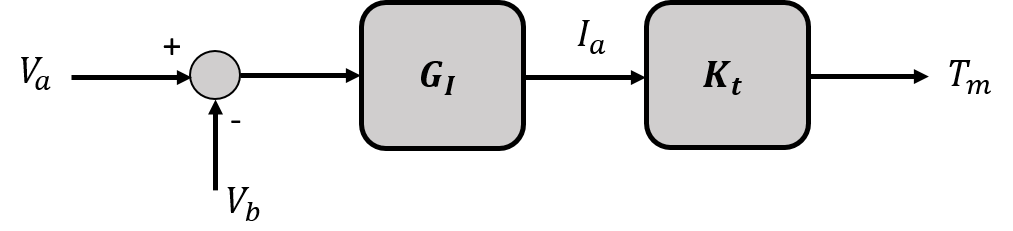
\includegraphics[scale=0.6]{figures/model2.png}
\caption{DC servomotor}
\label{model2}
\end{figure}

Using the previous expressions it is possible to associate the applied torque $T_{m}(s)$ to the angle position $\theta_{m}(s)$ (equations \ref{torque_frequency} and \ref{torque_frequency_G}).

\begin{equation}\label{torque_frequency}
T_{m}(s)\times I_{a}(s)= (s^{2}J_{e} + sD_{e})\theta_{m}(s)
\end{equation}

\begin{equation}\label{torque_frequency_G}
\theta_{m}(s)= G_{\theta}(s)\times T_{m}(s) , G_{\theta}(s)=\frac{1}{s^{2}J_{e} + sD_{e}}
\end{equation}

\begin{figure}[H]
\centering
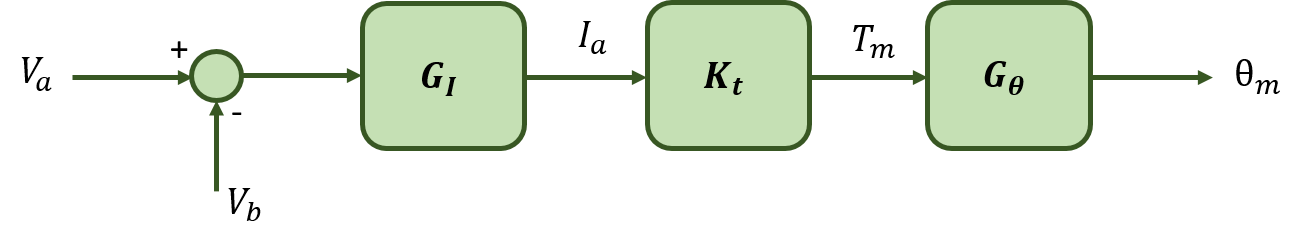
\includegraphics[scale=0.6]{figures/model3.png}
\caption{DC servomotor}
\label{model3}
\end{figure}

On the other hand, it is also possible to calculate the relation between the output theta and voltage. Thus, the comparison between the output and the input voltage allows the formation of a closed loop using a feedback (figure \ref{model4}).

\begin{equation}\label{feedback1}
v_{b}(t)= K_{b}\frac{\mathrm{d} \theta_{m}(t)}{\mathrm{d} t}
\end{equation}

\begin{equation}\label{feedback2}
V_{b}(s)= sK_{b}\theta_{m}(s)
\end{equation}

\begin{figure}[H]
\centering
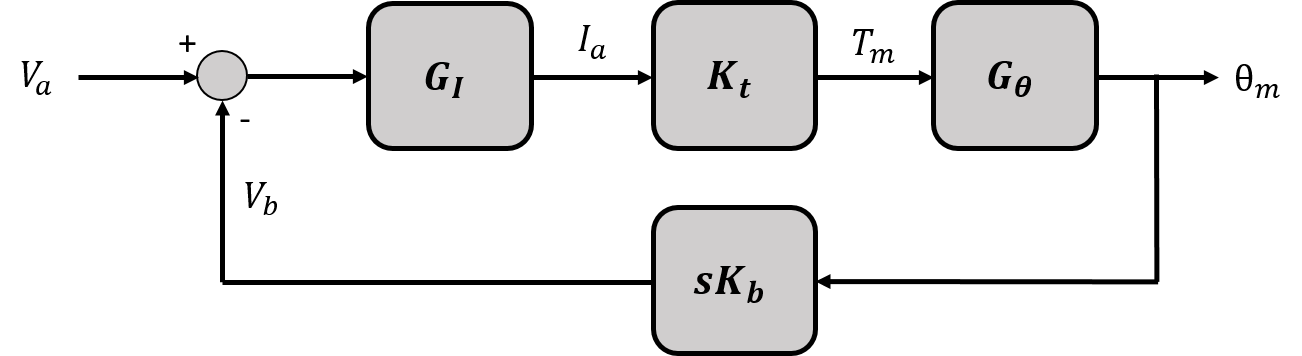
\includegraphics[scale=0.6]{figures/model4.png}
\caption{DC servomotor}
\label{model4}
\end{figure}


